\problemname{The Railway}

In these times of deregulated railways, Loke decides to start his own train company that will operate a certain railway line. Along this railway there are several stations, and one of Loke's first projects is to determine at which stations the important morning train should stop. Loke wants to base his decision on a large survey where he asked every potential passenger which stations they want to travel between and how long a travel time they can accept before choosing some other means of transport. Write a program that, based on this data, determines which stations the train should stop at to maximize the total number of passenger-kilometers.

\begin{figure}[!h]
\begin{center}
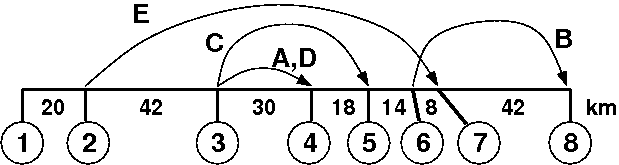
\includegraphics[width=0.7\textwidth]{jarnvagen.png}
\end{center}
\caption{The railway in the example. The arrows show the passengers' desired routes. Depending on the maximum travel time E chooses, different intermediate stations are optimal. In example 1, A, B, C, and D ride the train. In example 2, B and E ride. In example 3, A, D, and E ride. In example 4, A, B, D, and E ride.}
\label{fig1}
\end{figure}

\section*{Input}
The first line contains two integers $3\le N\ \le 20$, the number of stations, and $1 \le P \le 100$, the number of surveyed passengers. The stations are numbered in order along the track from the starting station 1 to the terminal station $N$ (the train must of course stop at these two stations). Then follows a line with $N-1$ integers in the range 2 to 1000, the length in kilometers of each segment between stations (see figure). All these numbers are for simplicity evenly divisible by two. The train normally always runs at 120 km/h, i.e. each kilometer takes exactly half a minute. Braking and acceleration, however, extend the time for each segment by one minute if the train stops at one of the segment's endpoint stations and two minutes if it stops at both endpoint stations. No extra time needs to be accounted for boarding and alighting; arrival time and departure time are the same. Finally follow $P$ lines with the survey answers, where each line contains the answers from one person: three integers $A$, $B$, and $M$, where $A$ is the station the person wants to depart from, $B$ is the station the person wants to travel to, and $M$ is the maximum travel time (in minutes) they can accept. The values satisfy $1\le A < B \le N$ and $2\le M\le 1000$.

\section*{Output}
Output an integer: the maximum number of passenger-kilometers that can be covered, i.e. for each
passenger whose requirements are met, sum up the distance they travel. 

Then output the timetable that achieves this maximum number of passenger-kilometers. It consists
of a line with two numbers for each station the train stops at: the station's number and the time
at which the train stops there. The train always starts at time 0. If there are multiple possible timetables,
the program should choose one that arrives at the terminal station as early as possible.

\section*{Scoring}
Your solution will be tested on a set of test groups.
To earn points for a group, you must pass all test cases in that group.

\noindent
\begin{tabular}{| l | l | p{12cm} |}
  \hline
  \textbf{Group} & \textbf{Points} & \textbf{Constraints} \\ \hline
  $1$    & $30$        & $N \leq 10$. \\ \hline 
  $2$    & $70$        & No additional constraints. \\ \hline 
\end{tabular}
